\chapter{Results}\label{results}

\todo[inline]{Revision 3}

In the previous chapter the research background and methodology adopted during the work were presented. This chapter summarises the papers that document the conducted research.

\section{Overview of research papers}\label{papers}

The research work has been published in two journal papers and four conference papers, one paper is currently ready for submission. In this section, papers that present the results of this thesis are summarised. Each summary includes: 
\begin{itemize}
	\itemsep1pt\parskip0pt\parsep0pt 
	\item Title 
	\item Authors and roles in the paper 
	\item Abstract of the paper
	\item Where the paper was published 
	\item A short description of how the paper relates to the research questions
\end{itemize}

Papers are reprinted in full in Part II of the thesis.

In addition to the papers presented in this section this PhD work has produced seven peer-reviewed papers. These papers present incremental achievements in research and have been summarised in in Appendix \ref{secondary-papers}

\section[P1: CroMAR: Mobile Augmented Reality for Supporting Reflection on Crowd Management][Paper 1]{Paper 1} \label{paper-1}

% PAPER 1
\emph{Title}: CroMAR: Mobile Augmented Reality for Supporting Reflection on Crowd Management

\emph{Authors}: Simone Mora, Alessandro Boron and Monica Divitini

\emph{Authors' contributions}: Mora led the research and the paper writing. He was actively involved in design, development, and evaluation of the system. Boron developed part of the described prototype and contributed to the paper with the description of the technical implementation. Divitini provided~general~supervision for the research and the paper writing. 

\begin{quote}
	\emph{Abstract:} This paper discusses the usage of Mobile Augmented Reality (MAR) to support reflection on past events, using reflection on crowd management as scenario. Computer based support to reflection generally relies on the visualization of information connected to the experience one is reflecting upon. Different metaphors have been adopted to support easy access to relevant information within the reflection process, e.g., timelines and word clouds. In this context, MAR represents an interesting alternative because it can be used to promote reflection in the specific location of the event by augmenting it with relevant information. In this way, the authors can expect the reflection process to be grounded in a context that helps to make sense of the information and reflect on alternative paths of action. The paper presents the scenario of usage, together with the design, development, and evaluation of the prototype, \emph{CroMAR}. Based on this experience, the authors identify challenges connected to the usage of Mobile Augmented Reality in terms of support for reflection, interaction, and design methodology. 
\end{quote}

\emph{Published in}: International Journal of Mobile Human Computer Interaction (IJMHCI), 2012

\emph{Description}: This paper initiates the design process of technology to support reflection (RQ2) by investigating the use of \emph{Mobile Augmented Reality} (MAR) to support debriefing after crowd management activities. To date, it is the first time that MAR is used for such purpose. Crowd management is a safety-critical activity performed by crisis workers during large public events (e.g. parades, sport events). It entails regulating flows of people to avoid the overcrowding of public places that might lead to dangerous consequences. 

Debriefing, as reported in Chapter \ref{csrl}, is a form of collaborative reflection in which a re-evaluation of experiences takes places. The paper presents \emph{CroMAR}, an iPad app designed by the authors, allows for browsing reflection-useful information. The system focuses on supporting navigation of reflection-useful information along the time and space dimension. Visualisation of information is provided in-situ, in a physical context that helps making sense of the information and reflect on alternative paths of actions. Also, the system provides support in involving others in the reflection process and in sharing of its outcome.

The proposed design has been implemented in a working prototype of an iPad app (Figure \ref{fig:cromar-prototype}), with focus on modularity and extensibility. The prototype has been evaluated in a focus group with experts (G2 in Table \ref{labtests}). The study highlights challenges in supporting reflective learning with MAR tools, with focus on user experience. First the research requires a better understanding of the conditions that makes MAR a better approach compared to other visualisation approaches (e.g.~maps, timelines). Second, it claims the need for providing scaffolding mechanisms to the reflection process; to make sure that relevant information for a given session is explored. Acknowledged by experts that the physical exploration of space provide scaffolding for exploration of information, it is necessary to study when it actually promotes reflection. 

\begin{figure}
	[tbh] \centering 
	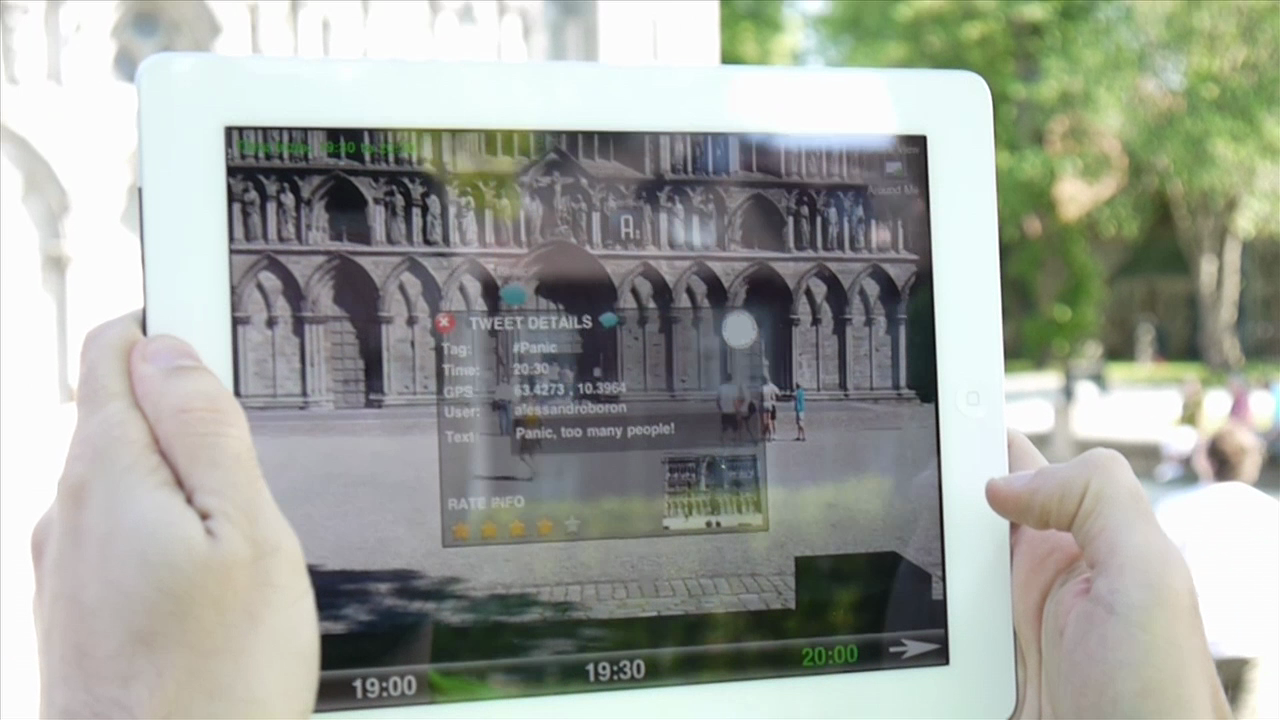
\includegraphics[width=1 
	\textwidth]{cromar_1stproto} \caption{\emph{CroMAR} early prototype} \label{fig:cromar-prototype} 
\end{figure}


The results from this paper have fed new design iterations for \emph{CroMAR}. The design of new functionalities has followed more closely the guidelines provided by the CSRL model that was being developed at the time. A new prototype of \emph{CroMAR} and its closer mapping to the CSRL model is described in P2.

%\emph{Relation to the research questions: } The paper started the investigation of RQ2, ``\RQii'' 

% Paper 2
\section[P2: Supporting Debriefing with Sensor Data: A Reflective Approach to Crisis Training][Paper 2]{Paper 2}\label{paper-2}

\emph{Title:} Supporting Debriefing with Sensor Data: A Reflective Approach to Crisis Training

\emph{Authors:} Simone Mora and Monica Divitini

\emph{Authors' contributions:} Mora led the research and the paper writing. He also led the design of the presented technology and directly implemented or supervised the implementation of the prototypes. Both authors attended the evaluation studies. Divitini provided general supervision for the research and the paper writing.

\begin{quote}
	\emph{Abstract:} In this paper we present our exploration into the use of sensor data to promote debriefing after training events simulating work experiences. In this way we address one of the core challenges of crisis training, namely the difficulty to exploit the full potential of training events, e.g. during drills. The paper is theoretically grounded in the theory of reflective learning. The theoretical understanding is used for informing the design of \emph{WATCHiT}, a wearable device for collecting sensor data during an event, and two applications for promoting debriefing in two different scenarios, \emph{CroMAR} and Procedure \emph{Trainer}. \emph{CroMAR} supports disaster managers during in-situ debriefing after large events, while Procedure \emph{Trainer} supports a team in reflecting after the simulation of a medical emergency procedure. The evaluation of the two applications shows that sensor data can be successfully used to support debriefing in both scenarios. Based on our experience, we draw lessons learned for the design of systems supporting debriefing in training events. 
\end{quote}

\emph{Published in:} Proceedings of Information Systems for Crisis Response and Management in Mediterranean Countries (ISCRAM-MED), 2014

\emph{Description:} This paper investigates how technology can improve the efficacy of debriefing with tools to capture data from work experiences (RQ1) and with user interfaces to browse information designed to facilitate triggering and supporting reflection activities (RQ2).

In this perspective, the paper presents an ecology of three technology tools to assist a wide range of scenarios. Also, in this work technology mapping with the CSRL model (Chapter \ref{csrl}) is made explicit. Two applications: \emph{CroMAR} and \emph{WATCHiT} also described in P1 and P3 and are presented in the last stage of their evolution. \emph{Trainer}, introduced in this paper, is a smartphone application to support a quick reflection session on the implementation of protocols (e.g. medical procedures) that can be done by the worker alone or in team. Building on results from tools evaluation during physical simulations, the paper presents lessons learnt about the design of systems to use of sensor data for supporting debriefing. 

\emph{First} it is acknowledged that sensor data has to be complemented by qualitative information in order to set the right focus for reflection and avoid over-sighting qualitative, yet critical aspects of the work that cannot be captured with quantitative methods.

\emph{Second} it suggests the use of \emph{visualisation} and \emph{storytelling} as mechanisms to promote sense-making processes for turning data into useful learning contents. Visualisation helps understanding the data by \emph{re-creating} a context that help spotting discrepancies with other sources and, in turn, triggers reflection. Storytelling happens when a visualisation need to be interpreted and explained both to oneself and to others, connecting data to the human memory of the event. Also, how to motivate the user in capturing data needed for visualisation and storytelling is an open challenge.

\emph{Third}, the proposed technologies aim at bringing debriefings out of the traditional office setting but not as substitutes, rather to complement the current practices by creating smooth transitions among different debriefing (and thus reflection) cycles. These propositions will guide future research to leverage sensor data in debriefings.

%\emph{Relation to the research questions:} The paper covers aspects of RQ1 ``\RQi'' and RQ2, ``\RQi''

% PAPER 3
\section[P3: WATCHiT: a modular and wearable tool for data collection in crisis management and training][Paper 3]{Paper 3}\label{paper-3}

\emph{Title:} WATCHiT: a modular and wearable tool for data collection in crisis management and training

\emph{Authors:} Simone Mora and Monica Divitini

\emph{Authors' contributions:} Mora led the research and the paper writing. He also presented the paper at the conference. Mora directly implemented or supervised the implementation of the prototypes. He also conducted the field studies and evaluations. Divitini provided general supervision for the research and the paper writing.

\emph{Published in:} Proceedings of the European Conference in Ambient Intelligence (AMI), 2014 

\begin{quote}
\emph{Abstract:} We present \emph{WATCHiT}, a prototype of sensor augmented wristband computer for data collection during crisis response work. During crises, information about the environment (e.g. to map the territory) and the rescuers (e.g. for assessment of workers' condition) offers help to support coordination of work, post-emergency debriefing and to build realistic training scenarios. Being each crisis nearly unique it is important to collect data from every single occurrence, yet it is difficult to foresee the type of data and context information that is relevant to capture. \emph{WATCHiT} features: (1) wearable sensors, (2) easy customisation of the type of information sensed, including both quantitative and qualitative data; (3) an intuitive, distraction-free user interface for controlling the data capturing procedure. Our design process has been driven by user studies during training events characterised by a high degree of realism; our prototype has been successfully evaluated with experts against technology acceptance. 
\end{quote}

\emph{Description:} This paper presents the design research that led the development of \emph{WATCHiT}, a wearable computer for data collection in-action during crisis response work (Figure \ref{fig:watchit-prototypes}). The design of \emph{WATCHiT} has been the primary mean of investigation for experience-capturing tools (RQ1). Field studies conducted by the authors (detailed in Chapter \ref{research}) have produced seven challenges for the design of technology tools to support data collection during real or simulated crisis. The drafted challenges highlight \emph{what} data are relevant to be captured and \emph{how} to collect them. Data captured can be used to feed reflection during debriefings (as shown in P2) as well as for helping coordination on the field and support decision-making processes.

The challenges drove the design of \emph{WATCHiT} by establishing three core requirements for the technology. \emph{WATCHiT} must be implemented to be \emph{wearable} -to achieve the highest degree of mobility in sensing-, \emph{modular} -to allow customisation of the type of data captured to specific crisis scenarios-; finally it has to feature a \emph{distraction-free user interface} to disrupt as little as possible the work. The requirements were gradually implemented in three prototyping iterations (Figure \ref{fig:watchit-prototypes}). Prototypes were built with the aid of rapid prototyping tools and techniques, in accordance with the investigation of RQ3.  Each prototype featured a mix of software and hardware technologies, and an increased degree of wearability. Modularity is implemented as an architectural choice with physical sensor modules that allow for transient customisation of sensing capabilities of the device.

\begin{figure}
	[tbh] \centering 
	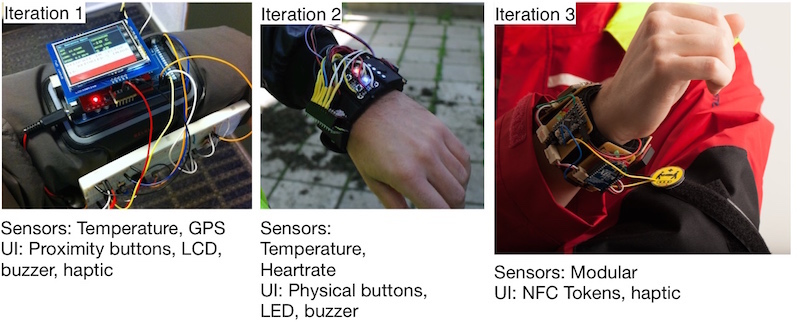
\includegraphics[width=1 
	\textwidth]{watchit_iterations} \caption{Three prototyping iterations for \emph{WATCHiT}} \label{fig:watchit-prototypes} 
\end{figure}

The requirement for distraction-free user interfaces has been implemented with the design of a novel sensing-based interface grounded on previous works on mnemonic body shortcuts and body-centric interaction \autocites{Guerreiro:2008wt}{Chen:2012wk}. In this work body shortcuts are specialised to assist data capturing processes. Areas on work uniforms and tools (identified by RFID tags) trigger digital operation when the worker puts \emph{WATCHiT} on. Each shortcut can be pre-configured to control the activation of specific sensors and to tag the data that is being captured with contextual information. User evaluations performed during physical simulations of crisis work have shown that the interaction technique is well accepted and \emph{WATCHiT} is suitable to be used during simulated crisis work.

\emph{WATCHiT} has been used to capture experiential data in order to feed technology-assisted debriefings thanks to the integration with \emph{CroMAR} and \emph{Trainer}, as described in P2. A new prototype and summative evaluation for the tool are described in P6.

%\emph{Relation to research questions:} The paper covers aspects of RQ1 ``\RQi''

%------PAPER 4
\section[P4: Don't Panic: Enhancing Soft Skills for Civil Protection Workers][Paper 4]{Paper 4}\label{paper-4}

\emph{Title:} Don't Panic: Enhancing Soft Skills for Civil Protection Workers

\emph{Authors:} Ines Di Loreto, Simone Mora and Monica Divitini

\emph{Authors' contributions:} All the co-authors contributed to the research.~Di Loreto, first author, led the game design and coordinated the paper writing. Mora contributed to game design with his knowledge of crisis training. He also contributed to the documentation of the work in the paper.~Divitini provided~general~supervision for the research and the paper writing.

\emph{Published in:} Proceedings of the International Conference on Serious Games Development Applications (SGDA), 2012 

\begin{quote}
	\emph{Abstract:} \emph{Don't Panic} is a serious game created to enhance soft skills in the crisis management field. The game is conceived to (i) add the fun element to training about stressful situations linked to panic management and (ii) teach skills such as communication styles, team management and coordination, time management, stress management and coping strategies. In this paper we present the first paper-based version of the game and its evaluation. The paper discusses the game design motivations, the methodological reasons behind its conception, and presents a pilot study. Results show that, even in its paper version, the game is a promising tool if linked with adequate and realistic procedures. This opens methodological questions about the role of computer based serious games. 
\end{quote}

\emph{Description:} This paper contributes to the design of novel sensing-based interfaces for supporting reflection (RQ2) by studying how serious games can be used as a tool to deliver realistic crisis work experiences. Serious games can complement other forms of training (for a list see Chapter \ref{crisis}) by enhancing workers' communication abilities, stress management and coping skills. The fun element typical of (computer or traditional) games can act as a motivation factor to engage workers in training. Furthermore games based on sensing-based interfaces can exploit tangible and embodied interaction to foster collaboration maintaining a link with the physical nature of crisis work.

After presenting the state of the art of serious games for crisis training, the paper dives into the description of \emph{Don't Panic}, a board game designed by the authors. The game aims at training soft skills in the management of situations where diffusion of panic might put the population at risk. During a game session different potential panicking events take place in the city represented on the board. The players have a limited time to calm down the situation, before the panic spreads and they lose the game. The game aims at teaching communication styles useful to manage crisis events but also foster team building. 

\begin{figure}
	[tbh] \centering 
	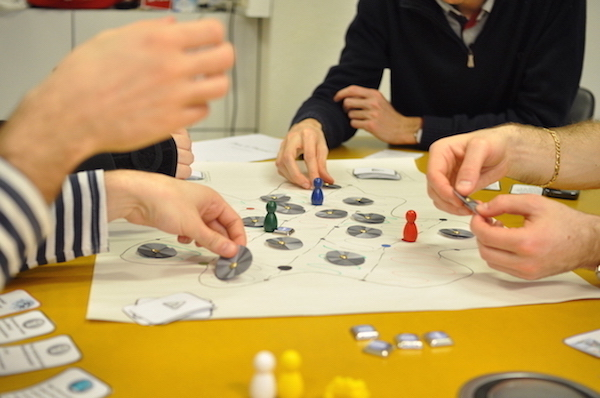
\includegraphics[width=1 
	\textwidth]{dp_mockup} \caption{Paper mockup of “Dont’ Panic”} \label{fig:dp-mockup} 
\end{figure}

The paper details game mechanics and rules. A paper prototype of \emph{Don't Panic} (Figure \ref{fig:dp-mockup}) is presented and evaluated in a pilot study with 10 crisis workers who played the game. The mockup, featuring no technology support, was used to validate game mechanics before moving proceeding to the design of a technology-augmented version of the game that is described in P5. The addition of technology can release the players from doing game management tasks which disrupted the game experience in the paper mockup. Moreover technology can be used to to add computer interactivity, for example by means of audio and graphic feedbacks. 

%\emph{Relation to the research questions: } The paper contributes to the investigation of RQ2, ``\RQii''

% PAPER 5

\section[P5: The interactive-token approach to board games][Paper 5]{Paper 5}\label{paper-5}

\emph{Title:} The interactive-token approach to board games

\emph{Authors:} Simone Mora, Ines Di Loreto and Monica Divitini

\emph{Authors' contributions:} Mora led the design and implementation work. He was also the main contributor of the paper. Di Loreto designed the board game that is used as example in the paper. Di Loreto and Mora jointly designed and attended evaluation studies. Divitini provided general supervision for the research and the paper writing.

\emph{Published in:} Ready for submission 

\begin{quote}
	\emph{Abstract:} Recent advances in interactive surfaces and Tangible User Interfaces have created a new interest in digital board games, aiming at mixing the benefits of traditional board games with the interactivity of video games. Within this strand of research we propose a new approach centred on the concepts of tokens, constraints, spatial expressions and interaction events. While mainstream solutions implement game interaction using interactive surfaces, our approach relies on physical manipulation of interactive objects on conventional surfaces. We illustrate the proposed approach by describing the design and development of a game for training of emergency workers. Building on feedbacks from user evaluation and our experience with the development, we outline design opportunities and challenges of the approach. 
\end{quote}

\emph{Description:} This paper presents a novel approach to the digitalisation of board games. As detailed in P4, board game dynamics can be adopted to generate realistic work experiences for training purposes. The approach presented in the paper can be used to drive the design of digital board games based on sensing-based interfaces. The design aims at enhancing interactivity and realism of the generated experiences, eventually pointing at triggering and supporting reflection (RQ2).

Rather than implementing games for interactive surfaces (e.g. touch-screens) the presented approach relies on the physical manipulation of interactive objects on conventional surfaces. After reviewing state of the art technology for digital board games, the approach is presented and grounded in existing frameworks of tangible user interfaces. To facilitate implementation of the approach into the design practice of digital board games a three-steps process is presented. 

The approach and process presented in this paper have been used to drive a new design iteration for the game introduced in P4., pointing out the role of technology as facilitator for generating engaging game experience and for supporting post-game reflection and mapping with the real work. 

In the new, technology-augmented prototype (Figure \ref{fig:dp-token}), social affordances of traditional board games, in terms of prompts for cooperation and discussion, are preserved. This is functional to the serious role of \emph{Don't Panic} as facilitator for storytelling and team building. At the same time the added computer interactivity provides a game experience which is more immersive and less disrupting compared to the paper mockup presented in P4. This allows for generating, by means of the game, a simulated work experience (management of panicking crowds) that re-create as much as possible conditions of emotional stress and decision making under time constraints, typical of real work. 

\begin{figure}
	[tbh] \centering 
	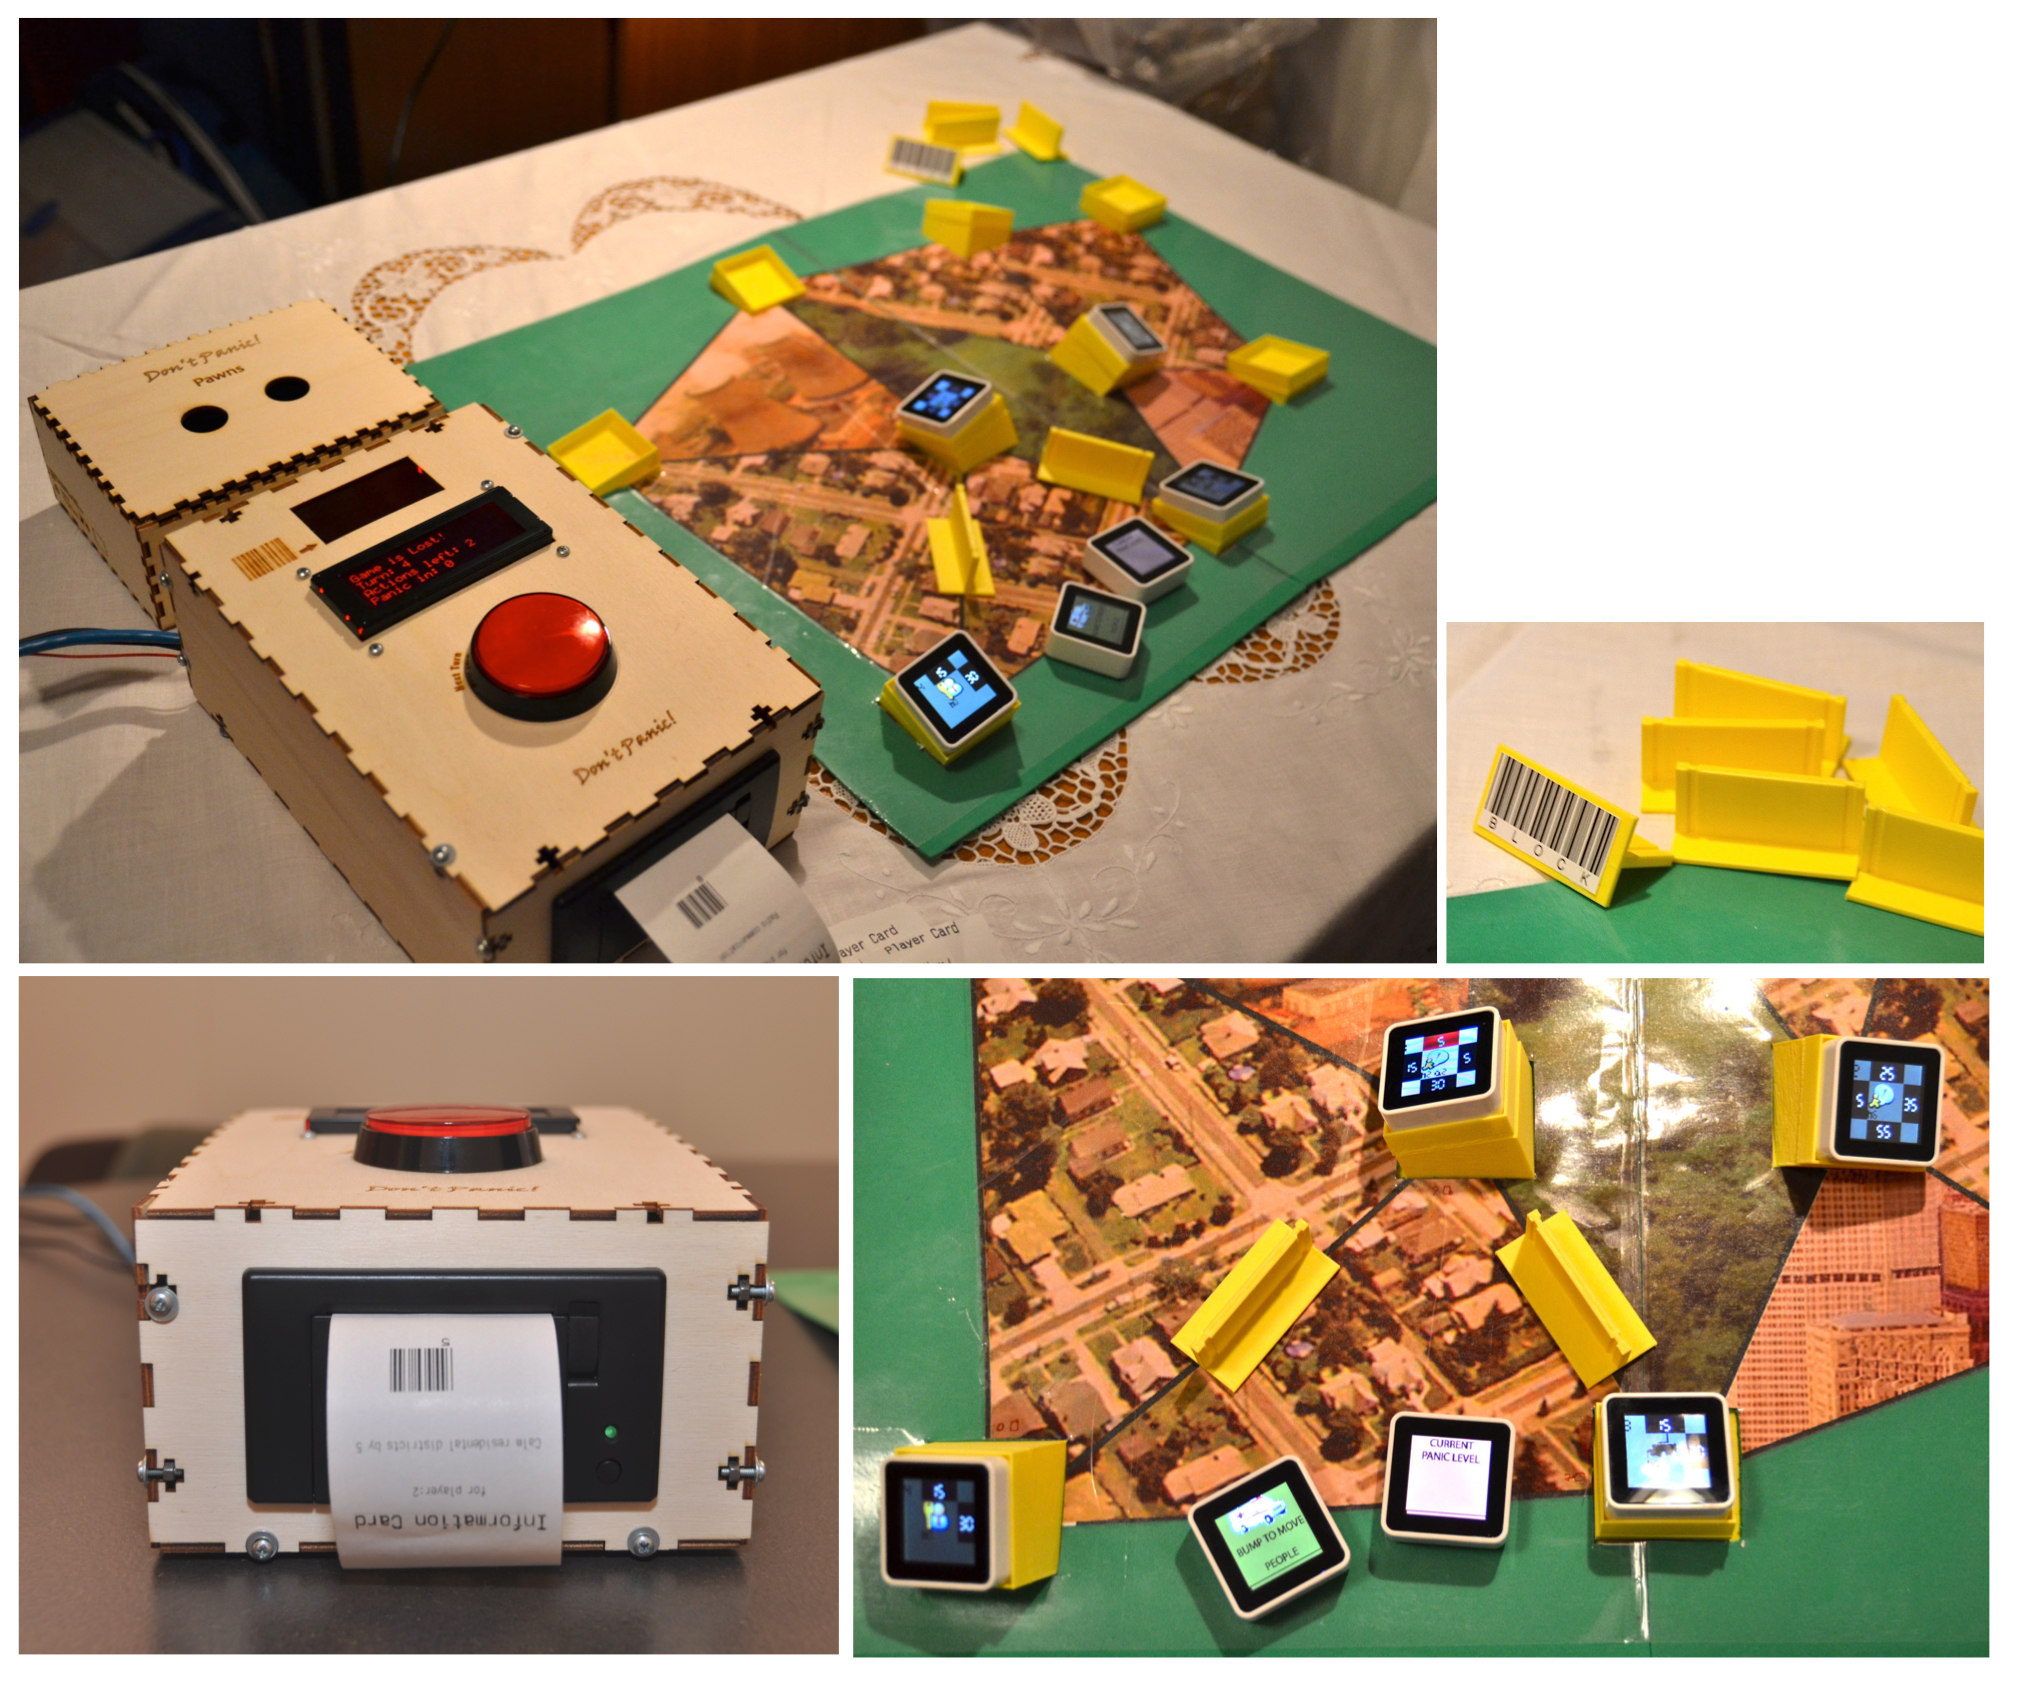
\includegraphics[width=1 
	\textwidth]{dp-multi} \caption{Technology-augmented “Don't Panic” working prototype} \label{fig:dp-token} 
\end{figure}

The paper also describes the technical challenges faced by the authors during the prototyping process, providing input to the study of RQ3. A mix of software, hardware, laser-cut and 3D printing techniques has been orchestrated in order to fully implement game dynamics and produce a prototype of a game that can be played for an entire session without major disruptions. Beside driving a new design iteration of \emph{Don't Panic} the approach proposed in the paper can inspire the design of digital board games for other domains.

%\emph{Relation to the research questions: } The paper contributes to the investigation of RQ2, ``\RQii'' and RQ3, ``\RQiii''

% PAPER 6

\section[P6: Context Becomes Content: Sensor Data for Computer Supported Reflective Learning][Paper 6]{Paper 6}\label{paper-6}

\emph{Title:} Context Becomes Content: Sensor Data for Computer Supported Reflective Learning

\emph{Authors:} Lars Müller, Monica Divitini, Simone Mora, Verónica Rivera-Pelayo and Wilhelm Stork

\emph{Authors' contributions:} Müller led the writing of the paper and contributed with one of the case studies. Mora designed the systems presented in the second case study. Mora also designed and conducted the evaluation of the system. Rivera-Pelayo contributed with state of the art about~the quantified self and to the methodological part. All the authors contributed to draw lessons learned and theoretical implications~from~the two~studies. Divitini and Stork contributed with supervision during the writing process.

\emph{Published in:} IEEE Transactions on Learning Technologies 
\begin{quote}
	\emph{Abstract:} Wearable devices and ambient sensors can monitor a growing number of aspects of daily life and work. We propose to use this context data as content for learning applications in workplace settings to enable employees to reflect on experiences from their work. Learning by reflection is essential for today's dynamic work environments, as employees have to adapt their behaviour according to their experiences. Building on research on computer-supported reflective learning as well as persuasive technology, and inspired by the Quantified Self community, we present an approach to the design of tools supporting reflective learning at work by turning context information collected through sensors into learning content. The proposed approach has been implemented and evaluated with care staff in a care home and voluntary crisis workers. In both domains, tailored wearable sensors were designed and evaluated. The evaluations show that participants learned by reflecting on their work experiences based on their recorded context. The results highlight the potential of sensors to support learning from context data itself and outline lessons learned for the design of sensor-based capturing methods for reflective learning. 
\end{quote}

\emph{Description:} This paper proposes the use of context data as content to support reflective learning in workplace settings. Three design decisions have to be made to turn context into content: \emph{what context} is relevant to be captured, \emph{how to capture} it and \emph{how to visualise} it to support reflection. While the elaboration of the first two decisions add to RQ1 by providing guidelines for the design of tools for experience collection, the third decision provides insights to RQ2 by guiding the design of interfaces that use data visualisation methods to sustain reflection. The first two decisions were already explored drafting design challenges for data capturing tools (P3). In this paper they are further elaborated.

Compared to P3 the paper adds that the decision of \emph{what context} is made harder by the unpredictability of outcomes typical of the reflective practice, and by the need for interpretation required by the unstructured nature of context data. Further, the paper groups context data in three categories: \emph{task}, \emph{affective} and \emph{social}. \emph{Task context} relates directly to the work process and is therefore easy to understand. \emph{Affective context} might work as a marker to recognise relevant episodes for reflection; because if something happens during the day, it will trigger an emotional reaction that can be captured with sensors. Finally \emph{social context} is important for many collaborative work practices since the interactions with other people (colleague, customers, patients) constitute an important aspect of many experiences to reflect upon. \emph{How to capture context} is also further elaborated in this paper. Three methods are proposed. Data can be \emph{self-reported} by the users, thus providing a subjective impression on an experience (e.g. by means of digital diaries). Data can be \emph{self-reported from third parties}, in this way an external perspective is made available to the reflecting person. Finally data can be captured \emph{automatically} by sensors and applications; for example by means of stress or activity-tracking sensors. Finally, the paper introduces a third design challenge connected to \emph{visualisation of context}. In order to be effective in triggering and sustaining a reflection sessions, data should be visualised from multiple perspectives. The social (comparing data over multiple users), spatial (the location data were captured) and historical perspectives (evolution of data samples over time) are considered as effective for reflection. 

These design dimensions are functional to build technology tools that implement the stages of the CSRL cycle (Chapter \ref{csrl}). While what context and how to capture it pertains designing of technology to support the \emph{plan and do work} stage of the model, \emph{how to visualise data} provides support for the subsequent stages of \emph{initiate reflection} and \emph{conduct reflection session}. Methods borrowed from persuasive technology and quantified self are presented to motivate the user in the data collection process

To evaluate the proposed approach the paper presents two case studies. The first case builds on the use of \emph{WATCHiT} (P3) and \emph{Trainer} (P2) to support reflection after crisis work. The second case is an application to support reflection for dementia carers designed by the the paper's co-authors. Field evaluations show that participants were able to learn from the visualised context. Capturing tools should be therefore be easy to adapt, in order to allow the users to deal with the unpredictability of relevance of the captured context. This challenge has been addressed in \emph{WATCHiT} (P3) by means of physical sensor modules.

%\emph{Relation to the research questions: } The paper dresses RQ1 ``\RQi'' and RQ2, ``\RQii''

%Paper 7
\section[P7: A Unified Architecture for Supporting Direct Tag-Based and Indirect Network-Based Resource Discovery][Paper 7]{Paper 7}\label{paper-7}

\emph{Title:} A Unified Architecture for Supporting Direct Tag-Based and Indirect Network-Based Resource Discovery

\emph{Authors:} Simone Mora and Babak Farshchian

\emph{Authors' contribution:} Mora conducted the design work and wrote the paper. Farshchian provided feedback throughout both the design and writing processes.

\emph{Published in:} Proceedings of the European Conference on Ambient Intelligence (AMI), 2010 
\begin{quote}
	\emph{Abstract:} Discovering and integrating ambient computational resources is a central topic in AmI. There are two major existing approaches: indirect network-based resource selection and direct tag-based resource identification. We motivate the need to integrate the two approaches through a scenario. We then present an architecture for a pluggable discovery system called UbiDisco. We demonstrate how UbiDisco implements a seamless integration of the two approaches at user interaction level through a framework for implementing discovery actions. 
\end{quote}

\emph{Description:} This work brings useful insights for the rapid prototyping approach adopted in this PhD (RQ3). As demonstrated in P2 and P6 the CSRL cycle is supported by a set of diverse technologies spanning from wearable and physical computers to apps for tablets and smartphones. Enabling workers to easily link those tools in order to allow data exchange is critical to build custom, scenario-specific ecologies of tools to support the different stages of the reflection cycle. Integrating different apps is technically complex since it involves serialisation of data, configuration of wireless networks and interaction of back-end services such as databases. From the perspective of the user it involves filling in configuration details. This activity might be very complex on mobile and wearable tools.

The paper presents a modular approach to software components for service discovery that blends the benefits of direct tag-based and indirect network-based discovery. The approach has been implemented in a middleware, called \emph{UbiDisco}, that allows for discovery and customisation of computational resources and support data exchange between heterogeneous systems. \emph{UbiDisco} is both a middleware and a collection of user interfaces for service discovery.

UbiDisco hinders the user from the complexity of configuring technical details by means of \emph{discovery actions}. The user can link two systems by reading a barcode or RFID tag which identifies the device/service and provide technical details for the configuration of the link. For example \emph{CroMAR} running on an iPad can be linked to \emph{WATCHiT}, by reading a barcode printed on the device hardware. In this way \emph{WATCHiT} and \emph{CroMAR} network addresses and protocols in use are exchanged between the two systems. \emph{WATCHiT} becomes a data provider for \emph{CroMAR} until a new \emph{discovery action} links \emph{WATCHiT} to a new system (e.g.~another instance of \emph{CroMAR} or \emph{Trainer}).

% \emph{Relation to the research questions: } The paper contributes to RQ3, ``\RQiii'' 
